\chapter{Topics in String Theory: Black Hole Entropy from Strings}

These notes follow Leonard Susskind's Lecture 6 in the supplementary 2011 Winter Topics in String Theory track, with curation by LazyingArt LLC. The lecture asks a concrete question: if a black hole has entropy, what microscopic objects carry it? The route is deliberately qualitative. One first identifies the relevant length scales and coupling constants, then compares the entropy of a black hole with the entropy of a highly excited string, and finally uses an adiabatic change of the coupling to connect the two descriptions.

\section{Entropy and the Microscopic Question}

Susskind begins by stripping the word \emph{entropy} back to its operational meaning. To say that a system has a large entropy is to say that it contains a large number of microscopic degrees of freedom which are too small and too numerous to track individually. A coarse-grained thermodynamic description tells us that these degrees of freedom exist, but does not tell us what they are.

The analogy is an ordinary fluid. Fluid dynamics describes velocity fields, densities, and macroscopic motion, but it does not by itself reveal the atomic structure of the fluid. Thermodynamics then tells us that the fluid has entropy, and this becomes evidence for microscopic structure beyond the macroscopic equations. Susskind's point is that the black-hole problem is of exactly the same kind. Bekenstein-Hawking entropy tells us that a black hole carries a vast amount of hidden information, but classical general relativity does not identify the microscopic carriers of that information.

Within string theory, the claim is that one can give a microscopic picture of those degrees of freedom. The lecture does not aim at a sharply exact formula with all numerical factors; it aims at the simplest argument that gets the order of magnitude and the scaling laws right.

\section{Planck Scale, String Scale, and the String Coupling}

The first task is to assemble the constants that the lecture will use. On the gravity side, the distinguished length scale is the Planck length,
\begin{equation}
\ell_p=\sqrt{\frac{G_N\hbar}{c^3}}.
\end{equation}
The lecture immediately passes to units in which
\begin{equation}
\hbar=c=1,
\end{equation}
so that Newton's constant is simply the Planck area:
\begin{equation}
\ell_p^2=G_N.
\end{equation}
In these units \(G_N\) has dimensions of area, which is why black-hole entropy is naturally measured as area in Planck units.

String theory brings in a different length scale, the string length \(\ell_s\). Susskind motivates it physically rather than axiomatically: if one heats up a string and looks at its oscillations, there is a characteristic wiggle scale, and that scale is \(\ell_s\). The string length is therefore the short-distance scale intrinsic to string dynamics, not the gravitational scale.

There is also a coupling constant, which the lecture describes operationally as the amplitude, or probability-like control parameter, for a string to split when it crosses itself. In cleaned notation it is best denoted by \(g_s\). Susskind's verbal usage shifts between probability language and amplitude language, but the role of the quantity is clear: it controls the emission of a small string, and in particular the emission of a graviton.

The lecture keeps \(g_s\) small. When \(g_s\ll 1\), the Planck length is correspondingly smaller than the string length. That hierarchy will matter when the black-hole and string descriptions are compared.

\section{From Photon Exchange to Graviton Exchange}

To motivate the relation between the coupling and Newton's constant, Susskind recalls the Feynman-diagram picture of ordinary electromagnetic force. One charged object emits a photon, another absorbs it, and the force is proportional to one factor of the charge from emission and one from absorption:
\begin{equation}
F_{\mathrm{EM}}\propto e^2.
\end{equation}

\begin{figure}[htbp]
\centering

\includegraphics[width=0.62\textwidth]{lecture_06_figure_03.png}
\caption{Photon-exchange Feynman sketch on the board. The irregular looped residue above the exchange diagram belongs to earlier board work and is not part of the reconstructed diagram.}
\end{figure}

\begin{figure}[htbp]
\centering
\begin{tikzpicture}[scale=1.0]
\draw[line width=0.8pt] (0,0) -- (0,3.2);
\draw[line width=0.8pt] (4.8,0) -- (4.8,3.2);
\draw[line width=0.8pt] plot[smooth] coordinates
{(0,1.55) (0.6,1.78) (1.2,1.30) (1.8,1.82) (2.4,1.28) (3.0,1.80) (3.6,1.32) (4.2,1.74) (4.8,1.55)};
\end{tikzpicture}
\caption{Clean reconstruction of the exchanged-photon sketch used to motivate the force law.}
\end{figure}

The string-theory version of gravity is then presented by analogy. If everything is made of strings, one object emits a graviton and another absorbs it. The force is therefore proportional to two powers of the string coupling:
\begin{equation}
F_{\mathrm{grav}}\propto g_s^2.
\end{equation}
But this cannot yet be Newton's constant, because \(g_s\) is dimensionless whereas \(G_N\) has dimensions of length squared. The only available length scale in the string description is \(\ell_s\), so dimensional analysis gives
\begin{equation}
G_N\sim g_s^2 \ell_s^2.
\end{equation}
Using \(\ell_p^2=G_N\), one immediately obtains the central relation
\begin{equation}
\ell_p=g_s \ell_s.
\end{equation}
This is one of the lecture's basic formulas: it ties together the gravitational scale, the string scale, and the strength of string interactions.

\section{Black-Hole Entropy}

Only after those scales are in place does Susskind turn to the entropy formulas themselves. For a Schwarzschild black hole, the Bekenstein-Hawking entropy is the horizon area measured in Planck units. Ignoring the standard factor of \(1/4\), the lecture uses
\begin{equation}
S_{BH}\sim \frac{A}{G_N}\sim \frac{A}{\ell_p^2}.
\end{equation}
The same formula can be rewritten in terms of the mass. Since
\begin{equation}
R_s=2MG_N,
\end{equation}
and the horizon area scales as \(A\sim R_s^2\), one finds
\begin{align}
A &\sim R_s^2 \sim (MG_N)^2,\\
S_{BH} &\sim \frac{A}{G_N}\sim \frac{M^2G_N^2}{G_N}\sim M^2G_N\sim M^2\ell_p^2.
\end{align}

\paragraph{Worked derivation.}
At the level of scaling used in the lecture, the passage from area form to mass form is:
\begin{enumerate}
\item \(S_{BH}\sim A/G_N\).
\item \(A\sim R_s^2\).
\item \(R_s\sim MG_N\), after dropping the factor of \(2\).
\item Therefore \(A\sim M^2G_N^2\).
\item Hence \(S_{BH}\sim M^2G_N\sim M^2\ell_p^2\).
\end{enumerate}

The important point is not the numerical coefficient but the scaling: black-hole entropy is quadratic in the mass, with the Planck area setting the gravitational unit.

\section{The Entropy of a Long Excited String}

Susskind then asks for the string-theory analogue. Start with a small string, add a large amount of energy, and it will generally not remain a neat simple loop. It becomes a tangled, random-walking ball of string. The entropy should therefore count the number of tangled configurations that are macroscopically hard to distinguish.

To make this count explicit, the lecture introduces a deliberately crude lattice model. Space is replaced by a lattice, and a string is modeled as a connected chain of links. The length of each link is taken to be the string length \(\ell_s\). In a two-dimensional toy lattice, each step has four possible continuations, even allowing the path to double back. Thus a string with \(n\) links has a number of states of order
\begin{equation}
\Omega_{\text{string}}\sim 4^n.
\end{equation}
Entropy is the logarithm of the number of macroscopically indistinguishable states, so
\begin{equation}
S_{st}\sim \log \Omega_{\text{string}}\sim n\log 4 \sim n.
\end{equation}
If \(L\) is the total length of the string measured along the curve, then
\begin{equation}
n=\frac{L}{\ell_s},
\end{equation}
and therefore
\begin{equation}
S_{st}\sim \frac{L}{\ell_s}.
\end{equation}

The lecture then converts this to a mass formula. In units with \(\hbar=c=1\), mass has dimensions of inverse length, so one lattice link carries mass of order
\begin{equation}
m_{\text{link}}\sim \frac{1}{\ell_s}.
\end{equation}
A string with \(n\) links therefore has total mass
\begin{equation}
M\sim \frac{n}{\ell_s}\sim \frac{L}{\ell_s^2}.
\end{equation}
Equivalently,
\begin{equation}
L\sim M\ell_s^2.
\end{equation}
Substituting back into the entropy formula yields
\begin{equation}
S_{st}\sim M\ell_s.
\end{equation}

\paragraph{Worked derivation.}
The long-string counting can be summarized in the same style as the lecture:
\begin{enumerate}
\item Model the excited string as a chain of \(n\) lattice links of size \(\ell_s\).
\item Count states as \(\Omega\sim 4^n\) in the two-dimensional toy model.
\item Take the logarithm: \(S_{st}\sim n\).
\item Replace \(n\) by \(L/\ell_s\), so \(S_{st}\sim L/\ell_s\).
\item Use \(m_{\text{link}}\sim 1/\ell_s\), hence \(M\sim n/\ell_s\sim L/\ell_s^2\).
\item Eliminate \(L\): \(L\sim M\ell_s^2\).
\item Conclude that \(S_{st}\sim M\ell_s\).
\end{enumerate}

This is where the lecture slows down on purpose. The black-hole formula and the string formula look suggestive, but they do not match:
\begin{equation}
S_{BH}\sim M^2\ell_p^2,
\qquad
S_{st}\sim M\ell_s.
\end{equation}
The mismatch is the next piece of the story. It tells us that the weakly coupled long string is not yet the macroscopic black hole whose entropy we want to understand.

\section{Turning on Gravity: From String to Black Hole}

The next move is dynamical rather than algebraic. Susskind asks us to imagine that the string coupling \(g_s\) can be varied adiabatically, like slowly turning a control knob. Start at very small coupling, even \(g_s=0\), so that gravity is negligible. At that end of parameter space a highly excited object is simply a long tangled string, not a black hole.

Now increase \(g_s\), keeping \(\ell_s\) fixed. Since
\begin{equation}
G_N\sim g_s^2\ell_s^2,
\end{equation}
gravity becomes stronger. The tangled string begins to pull itself together. Its gravitational potential energy is negative, so as the object contracts its total energy decreases. The mass therefore decreases while the density increases. If the contraction continues far enough, the object's size eventually drops below its Schwarzschild radius. At that point the description changes: the object becomes a black hole.

This is not merely a one-way process. If one begins with a black hole and slowly turns the coupling back down, there is eventually not enough gravity to hold the object in its black-hole form, and the system returns to a string description. Susskind emphasizes that, for fixed total mass in a fixed volume, the maximal-entropy string state is still essentially one long string rather than a large collection of small disconnected strings. The lecture does not derive that claim here, but it uses it as part of the intuition that the black-hole state and the long-string state are two descriptions of the same high-entropy object in different regions of parameter space.

\section{The Horizon Picture, the Transition Point, and Adiabatic Invariance}

Once the string has turned into a black hole, the lecture asks what becomes of the stringy degrees of freedom from the viewpoint of an outside observer. The answer is not that they simply disappear behind the horizon. In the outside description, they pile up on or near the horizon.

\begin{figure}[htbp]
\centering

\includegraphics[width=0.72\textwidth]{lecture_06_figure_04.png}
\caption{Near-horizon schematic for stringy degrees of freedom. The board drawing is qualitative: it indicates localization on or near the horizon, not a precise coordinate construction.}
\end{figure}

\begin{figure}[htbp]
\centering
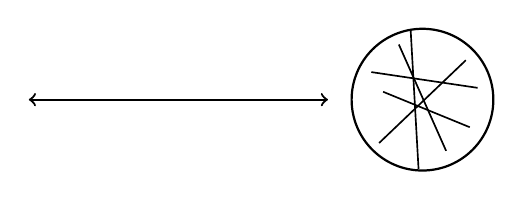
\begin{tikzpicture}[scale=1.0]
\draw[<->, line width=0.8pt] (-3.0,0) -- (0.8,0);
\draw[line width=0.8pt] (2.0,0) circle (0.9);
\draw[line width=0.6pt] (1.45,-0.55) -- (2.55,0.50);
\draw[line width=0.6pt] (1.50,0.10) -- (2.60,-0.35);
\draw[line width=0.6pt] (1.70,0.70) -- (2.30,-0.65);
\draw[line width=0.6pt] (1.35,0.35) -- (2.70,0.15);
\draw[line width=0.6pt] (1.85,0.88) -- (1.95,-0.88);
\end{tikzpicture}
\caption{Cleaned qualitative reconstruction of the near-horizon sketch.}
\end{figure}

For a large black hole, much larger than the string scale, this stringy structure is only a small amount of fuzz on the horizon. But Susskind then asks a sharper question: what happens when the black hole is so small that its Schwarzschild radius becomes comparable to the size of the string loops? At that point the black-hole description itself loses meaning. This defines the transition point:
\begin{equation}
R_s\sim \ell_s.
\end{equation}

\begin{figure}[htbp]
\centering

\includegraphics[width=0.72\textwidth]{lecture_06_figure_05.png}
\caption{Blackboard comparison of black-hole and string entropy formulas. The lower line begins with \(R_s=\); the completed transition condition is reconstructed from the surrounding argument rather than read directly from the frame.}
\end{figure}

Near the board screenshot, the cleaned comparison is
\begin{align}
S_{BH} &\sim \frac{A}{\ell_p^2}\sim M^2\ell_p^2,\\
S_{st} &\sim \frac{L}{\ell_s}\sim M\ell_s.
\end{align}
The transition condition can be rewritten in several equivalent forms. Since \(R_s\sim MG_N\), one has
\begin{equation}
MG_N\sim \ell_s.
\end{equation}
Using \(G_N=\ell_p^2\), this becomes
\begin{equation}
M\ell_p^2\sim \ell_s.
\end{equation}
Finally, with \(\ell_p=g_s\ell_s\),
\begin{align}
M(g_s^2\ell_s^2) &\sim \ell_s,\\
Mg_s^2\ell_s &\sim 1.
\end{align}
The board algebra in the lecture becomes verbally messy at this point, so it is best to present the cleaned result only at the level of scaling.

The final ingredient is adiabatic invariance. If one varies a control parameter slowly enough and does not cross a genuine phase transition, the entropy does not change. In the present context that statement is used as
\begin{equation}
\Delta S=0
\qquad
\text{under an adiabatic change of } g_s.
\end{equation}
This gives the strategy of the whole lecture:
\begin{enumerate}
\item Start with a black hole of given mass at some coupling.
\item Decrease the coupling adiabatically.
\item At the transition point the object becomes a string.
\item Compute the entropy in the string description.
\item Because the entropy has not changed, infer the entropy of the original black hole.
\end{enumerate}
The lecture stops just after laying out this strategy. The final assembly of the formulas is deferred to the next lecture.

\section{Summary}

The lecture's logical spine is simple even though the ingredients take time to assemble. Entropy is hidden information, so black-hole entropy demands microscopic degrees of freedom. String theory supplies a candidate microscopic description in terms of highly excited long strings. The essential formulas are
\begin{equation}
\ell_p^2=G_N,
\qquad
\ell_p=g_s\ell_s,
\qquad
S_{BH}\sim M^2\ell_p^2,
\qquad
S_{st}\sim M\ell_s.
\end{equation}
At weak coupling these do not match directly, so one turns the coupling into a dynamical dial. As \(g_s\) increases, a long string contracts and becomes a black hole; as \(g_s\) decreases, the black hole returns to a string. The crossover occurs when \(R_s\sim \ell_s\), or equivalently \(Mg_s^2\ell_s\sim 1\). Because entropy is unchanged under an adiabatic variation of the coupling, the entropy computed in the string description can be carried back to the black-hole description. That is the argument promised by the lecture, and its completion lies immediately ahead.